\documentclass[tikz,border=2pt]{standalone}
\usepackage{amsmath,amssymb}
\usepackage{pgfplots}
\pgfplotsset{compat=1.18}
\usetikzlibrary{arrows.meta}

\begin{document}
% x^2 sin(1/x) is squeezed between -x^2 and x^2 on [-0.2, 0.2]; both bounds tend to 0 at 0.
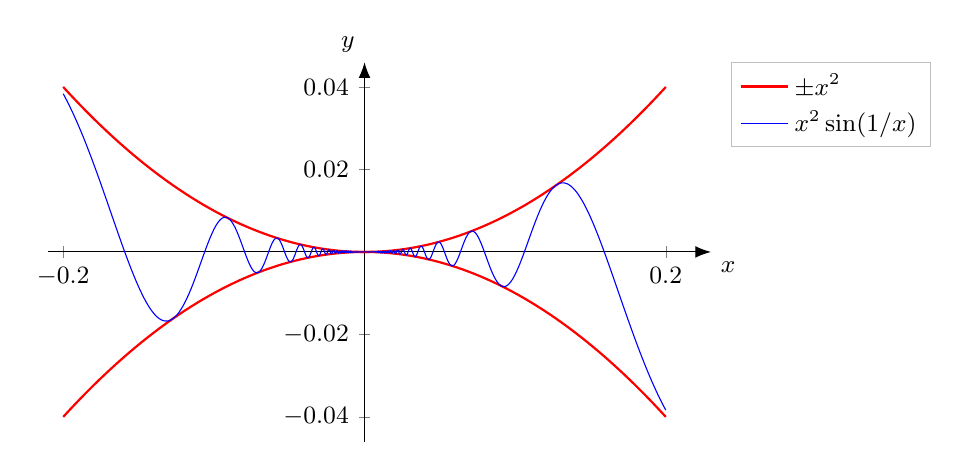
\begin{tikzpicture}[every node/.style={font=\small}]
	\begin{axis}[
		width=10cm, height=6.4cm,
		axis lines=middle, axis line style={-{Latex[length=2mm]}},
		xmin=-0.21, xmax=0.23, ymin=-0.046, ymax=0.046,
		xtick={-0.2,0.2}, ytick={-0.04,-0.02,0.02,0.04},
		legend pos=outer north east, legend style={font=\small, draw=gray!50, fill=white},
		legend cell align={left},
		tick label style={font=\small, /pgf/number format/fixed},
		scaled y ticks=false,
		xlabel={$x$}, ylabel={$y$},
		xlabel style={below right}, ylabel style={above left},
		clip=false
		]
		\addplot[red, thick, domain=-0.2:0.2, samples=100] {x^2};
		\addlegendentry{$\pm x^2$}
		\addplot[red, thick, domain=-0.2:0.2, samples=100, forget plot] {-x^2};
		\addplot[blue, domain=-0.2:0.2, samples=1500] {x^2*sin(deg(1/x))};
		\addlegendentry{$x^2\sin(1/x)$}
	\end{axis}
\end{tikzpicture}
\end{document}
